\documentclass[12pt]{article}

% ----------------------------------------------------------------------
% Define external packages, language, margins, fonts, new commands 
% and colors
% ----------------------------------------------------------------------
\usepackage[utf8]{inputenc} % Codification
\usepackage[english]{babel} % Writing idiom
\usepackage{multirow}
\usepackage[export]{adjustbox} % Align images
\usepackage{amsmath} % Extra commands for math mode
\usepackage{amssymb} % Mathematical symbols
\usepackage{anysize} % Personalize margins
    \marginsize{2cm}{2cm}{2cm}{2cm} % {left}{right}{above}{below}
\usepackage{appendix} % Appendices
\usepackage{cancel} % Expression cancellation
\usepackage{caption} % Captions
    \captionsetup{labelfont={bf}}
\usepackage{cite} % Citations, like [1 - 3]
\usepackage{color} % Text coloring
\usepackage{fancyvrb}
\usepackage{fancyhdr} % Head note and footnote
    \pagestyle{fancy}
    \fancyhf{}
    %\fancyhead[L]{\footnotesize Graduating } % Left of Head note
    \fancyhead[R]{\footnotesize UNYT} % Right of Head note
    \fancyfoot[L]{\footnotesize Graduating Project} % Left of Footnote
    \fancyfoot[C]{\thepage} % Center of Footnote
    \fancyfoot[R]{\footnotesize Department of Computer Science} % Right of Footnote
    \renewcommand{\footrulewidth}{0.4pt} % Footnote rule
\usepackage{float} % Utilization of [H] in figures
\usepackage{graphicx} % Figures in LaTeX
\usepackage[colorlinks = true, plainpages = true, linkcolor = istblue, urlcolor = istblue, citecolor = istblue, anchorcolor = istblue]{hyperref}
\usepackage{indentfirst} % First paragraph
\usepackage[super]{nth} % Superscripts
\usepackage{siunitx} % SI units
\usepackage{subcaption} % Subfigures
\usepackage{titlesec} % Font
    \titleformat{\section}{\Large\bfseries}{\thesection}{1em}{}
    \titleformat{\subsection}{\large\bfseries}{\thesubsection}{1em}{}
    \titleformat{\subsubsection}{\normalsize\bfseries}{\thesubsubsection}{1em}{}
    \fancyfoot[C]{\thepage}
% Random text (not needed)
\usepackage{duckuments}
\usepackage{booktabs}
\usepackage{url}
\usepackage{graphicx}

% New and re-newcommands
\newcommand{\HRule}{\rule{\linewidth}{0.5mm}} % Specific rule definition
\renewcommand{\appendixpagename}{\LARGE Appendices}
\newcommand{\sectiononlytoc}[1]{%
    \par
    \refstepcounter{section}%
    % Don't print sectional unit; just add to ToC and update the Left header
    \addcontentsline{toc}{section}{\protect\numberline{\thesection}#1}%
    %\fancyhead[L]{#1}% Add chapter title in Left header
}

% Colors
\definecolor{istblue}{RGB}{3, 171, 230}
\definecolor{dkgreen}{rgb}{0,0.6,0}
\definecolor{gray}{rgb}{0.5,0.5,0.5}

%%%%%%%%%%%%%%%%%%%%%%%%%%%%%%%%%%%%%%%%%%%%%%%%%%%%%%%%%%%%%%%%%%%%%%%%
%                                 Document                             %
%%%%%%%%%%%%%%%%%%%%%%%%%%%%%%%%%%%%%%%%%%%%%%%%%%%%%%%%%%%%%%%%%%%%%%%%
\begin{document}

% ----------------------------------------------------------------------
% Cover
% ----------------------------------------------------------------------
\begin{center}
    \mbox{}\\[2.0cm]
    \LARGE Enabling Multilingual Communication: Automated Lip-synchronization Dubbing for Albanian Videos
\end{center}

\vspace{10cm}

\begin{center}
    \Large ALDO DIKU
\end{center}

\vspace{5cm}

\begin{center}
    \Large UNIVERSITY OF NEW YORK TIRANA
\end{center}
\begin{center}
    \large \Large JULY 2025
\end{center}
\thispagestyle{empty}

\setcounter{page}{0}

\newpage
% ----------------------------------------------------------------------
% APPROVAL PAGE
% ----------------------------------------------------------------------
\noindent This is to certify that I have read this project and that, in my opinion, it is fully adequate, in scope and quality, as a thesis for the degree of Bachelor of Arts in Computer Science.

\vspace{4cm}

\noindent
(Title and Name) \hspace{4cm} \\
(Project Advisor) \hspace{2cm} \underline{\hspace{2cm}} \hspace{1cm} \underline{\hspace{8cm}}

\vspace{3cm}

\noindent This is to confirm that this thesis complies with all the standards set by the Department of Computer Science of University of New York Tirana.

\vspace{2cm}

\noindent Date: \hspace{5cm} \hfill Seal/Signature: \hspace{5cm}

\setcounter{page}{1}

\newpage

% ----------------------------------------------------------------------
% PLAGARIZM CLEARANCE PAGE
% ----------------------------------------------------------------------
\noindent I hereby declare that all information in this document has been obtained and presented in accordance with academic rules and ethical conduct. I also declare that, as required by these rules and conduct, I have fully cited and referenced all material and results that are not original to this work.

\vspace{2cm}

\noindent \hspace{7.5cm} First Name, Last Name:\\
\\
\vspace{1.0cm}
\noindent \hspace{7.3cm} \text{Signature:} % NO CLUE WHY THIS IS 7.3 AND NOT 7.5 LIKE ABOVE

\setcounter{page}{2}

\newpage

% ----------------------------------------------------------------------
% ABSTRACT
% ----------------------------------------------------------------------
\sectiononlytoc{Abstract}
\begin{center}
    
    \vspace{0.5cm}
    
    ABSTRACT
    
    \vspace{1cm}
    
    \centering{ ENABLING MULTILINGUAL COMMUNICATION: AUTOMATED LIP-SYNCHRONIZATION DUBBING FOR ALBANIAN VIDEOS}
    
    \vspace{1cm}
    
    Diku, Aldo.
    
    BA. in Computer Science
    
    Thesis Advisor: Prof. Miralda Çuka
    
    June 2025, 20 pages
    
    \vspace{1cm}
\end{center}

\noindent Using available methods and tools (which i will mention when i gather all the tools and methods) to create lip-synced dubbed videos from an albanian video input and outputting a video of the same speaker in another language with the lips moving according to that languages movements. 
    
\vspace{1cm}
    
\noindent Keywords: Lip-sync, dubbing, albanian language

\newpage

% ----------------------------------------------------------------------
% Acknowledgements
% ----------------------------------------------------------------------

\sectiononlytoc{Acknowledgements}

First and foremost, I would like to express my sincere gratitude to my advisor, Professor Miralda Çuka, for their invaluable guidance, unwavering support, and insightful feedback throughout this project. Their expertise and encouragement were instrumental in shaping this work.

Finally, I am grateful for the support of my family and friends. Something something a little bit longer and better made.

\newpage


% ----------------------------------------------------------------------
% Contents
% ----------------------------------------------------------------------
\tableofcontents 

\newpage

% ----------------------------------------------------------------------
% Body
% ----------------------------------------------------------------------
\section{Introduction}
\subsection{Background of the study}
The increasing globalisation of online content consumption presents a significant challenge for video creators aiming to reach diverse audiences, thereby creating the need to produce multilingual versions of their work. Being able to make only one video and have it transform into multiple languages will help creators but also the target audience as well. Cutting down on the time and money it takes to make two or more videos with the same subject but in different languages. One such case is a youtube creator named der8auer from Germany, for the same topic he creates two videos, one in english and one in german. Sometimes his videos are quite long and having to do them again in another language will tire you out. Having a model that can take your video, translate it into another language and synchronize your lips to the movement of the language of your choosing would be a tool in your arsenal. Some of the usages of this lip-sync dubbing technology are: video dubbing and translation, real-time Face-to-Face translation that will be possible in the future and multilingual communication, gaming and virtual environments reduced cost and labor and time in this case, entertainment and content creation, speech recognition and lip-reading. Film, entertainment and media production. Education and training videos, especially in cases where there is a diverse workforce. It also has promising applications in areas for speech therapy, language learning and assistive communication devices for individuals with hearing impairments \cite{biomedinformatics4010023}. Advancements in Machine Learning (ML) have made it possible to have Automatic Speech Recognition (ASR) 

\subsection{How lip synchronization works}
Phonemes are the distinct units of sound in speech, and visemes are visual representations of phonemes. Think phonemes as the audio and visemes as the video. Visemes serve to map sounds (phonemes) to corresponding mouth positions or shapes. The goal is to go from the audible  to the visual (visemes). Visemes group similar-looking mouth shapes, which reduces the complexity required for animation. Relating the extracted audio features to the corresponding visual mouth shapes and facial expression. Mapping phonemes down to a smaller number of visemes gives artists fewer expressions to pose. The history of lip-syncing comes from animation and in particular two-dimensional cartoons where artists had to make facial movement according to the sounds of speech \cite{game-lipsynch}. Lip-synchronization is a field that has been studied since 1994 \cite{earliest-lip-synch}, where Automatic lip-sync (ALS) could be used for animating cartoons realistically making the mouth movement more smoother and have a more natural feel and could also help in aiding people with hearing disability. Later in 1997 a new method was proposed where they used Fast Fourier Transform (FFT) for speech signal analysis, statistical measures called "moments" are used to describe the shape of the FFT. Mouth parameter measurements are used to measure the jaw position, the height of the maximum vertical opening between the lips and horizontal opening of the lips. This method did not require phonemic analysis or prior knowledge of the speech content. ObamaNet was an innovative architecture released in 2017, it used a time-delayed Long Short-Term Memory (LSTM) network to produce synchronized lip-synch videos. The network learned to map raw audio feature to corresponding mouth shapes based on hours of high-quality videos of a specific target person \cite{ObamaNet}. Convolutional Neural Networks (CNN) played an important role in lip-synchronization as it helped in feature extraction for visual features, and image processing and generation. CNNs are often used with other models like LSTM blocks, or encoder and discriminator networks based on a Generative Adversarial Networks (GAN). A study by Pawar et al. (2024) focused on Marathi, an Indian language which has a shortage of datasets, similar to that of the Albanian language \cite{PAWAR2024100084}. Integrating CNNs with adversarial training and including RNN-based architectures, specifically LSTM for lip-synch generation, Song et al. (2019), Sadoughi et al. (2021) and Li et al (2021) also used a combination of CNN, RNN, GANs and LSTMs \cite{Audio-driven-facial-animation} \cite{Li_2021}. Another similar study by Exarchos et al. (2024) for lip-reading in Greek language tackeld the scarcity of datasets available. The study proposed a combination of 3D CNNs and LSTM networks for word recognition from lip movements.  

\section{Methodology}
A key limmitation encountered was the lack of suitable Albanian video datasets, specifically open-license content with direct-to-camera speech, reflecting the broader challange of working with low-resource languages in multimedia applications. To address the first issue, custom video contennt was created featuring self-recorded footage in a one by one aspect ratio and lowest camera setting to save. The first step for this project was the data creation, seeing as there is not a lot of free and publicly available free-use content I can use we had to create the data myself. Videos were filmed 50 centimeters away from the recording device, different surrounding light, camera position (slightly down or up), shaved and unshaved faces were recorded to check the quality of the lip-synching models if they could simulate the bearded area around the lips. Five videos were created with moving backgrounds to check how the lip-synching model with handle changing background. One of the videos contains the head moving and lips being out of clear view, checking the limits of the model. Videos were recorded at 1440x1440 resolution (1:1 aspect ratio) at 30 frames per second, with durations ranging from 10 seconds up till 5 minutes. The study at (citation needed for the optimal length of time of the videos) found that the optimal length time was for videos with one word in them. To adapt to this, a script was made to create small chunks of videos to be closer to that optimal format. Videos could have been created by following and reading a script thereby avoiding the transcipiton step, however we want to create a workflow that will take any video of an albanian speaker and turn it into a dub lip synched video.

\begin{figure}[h!]
    \centering
    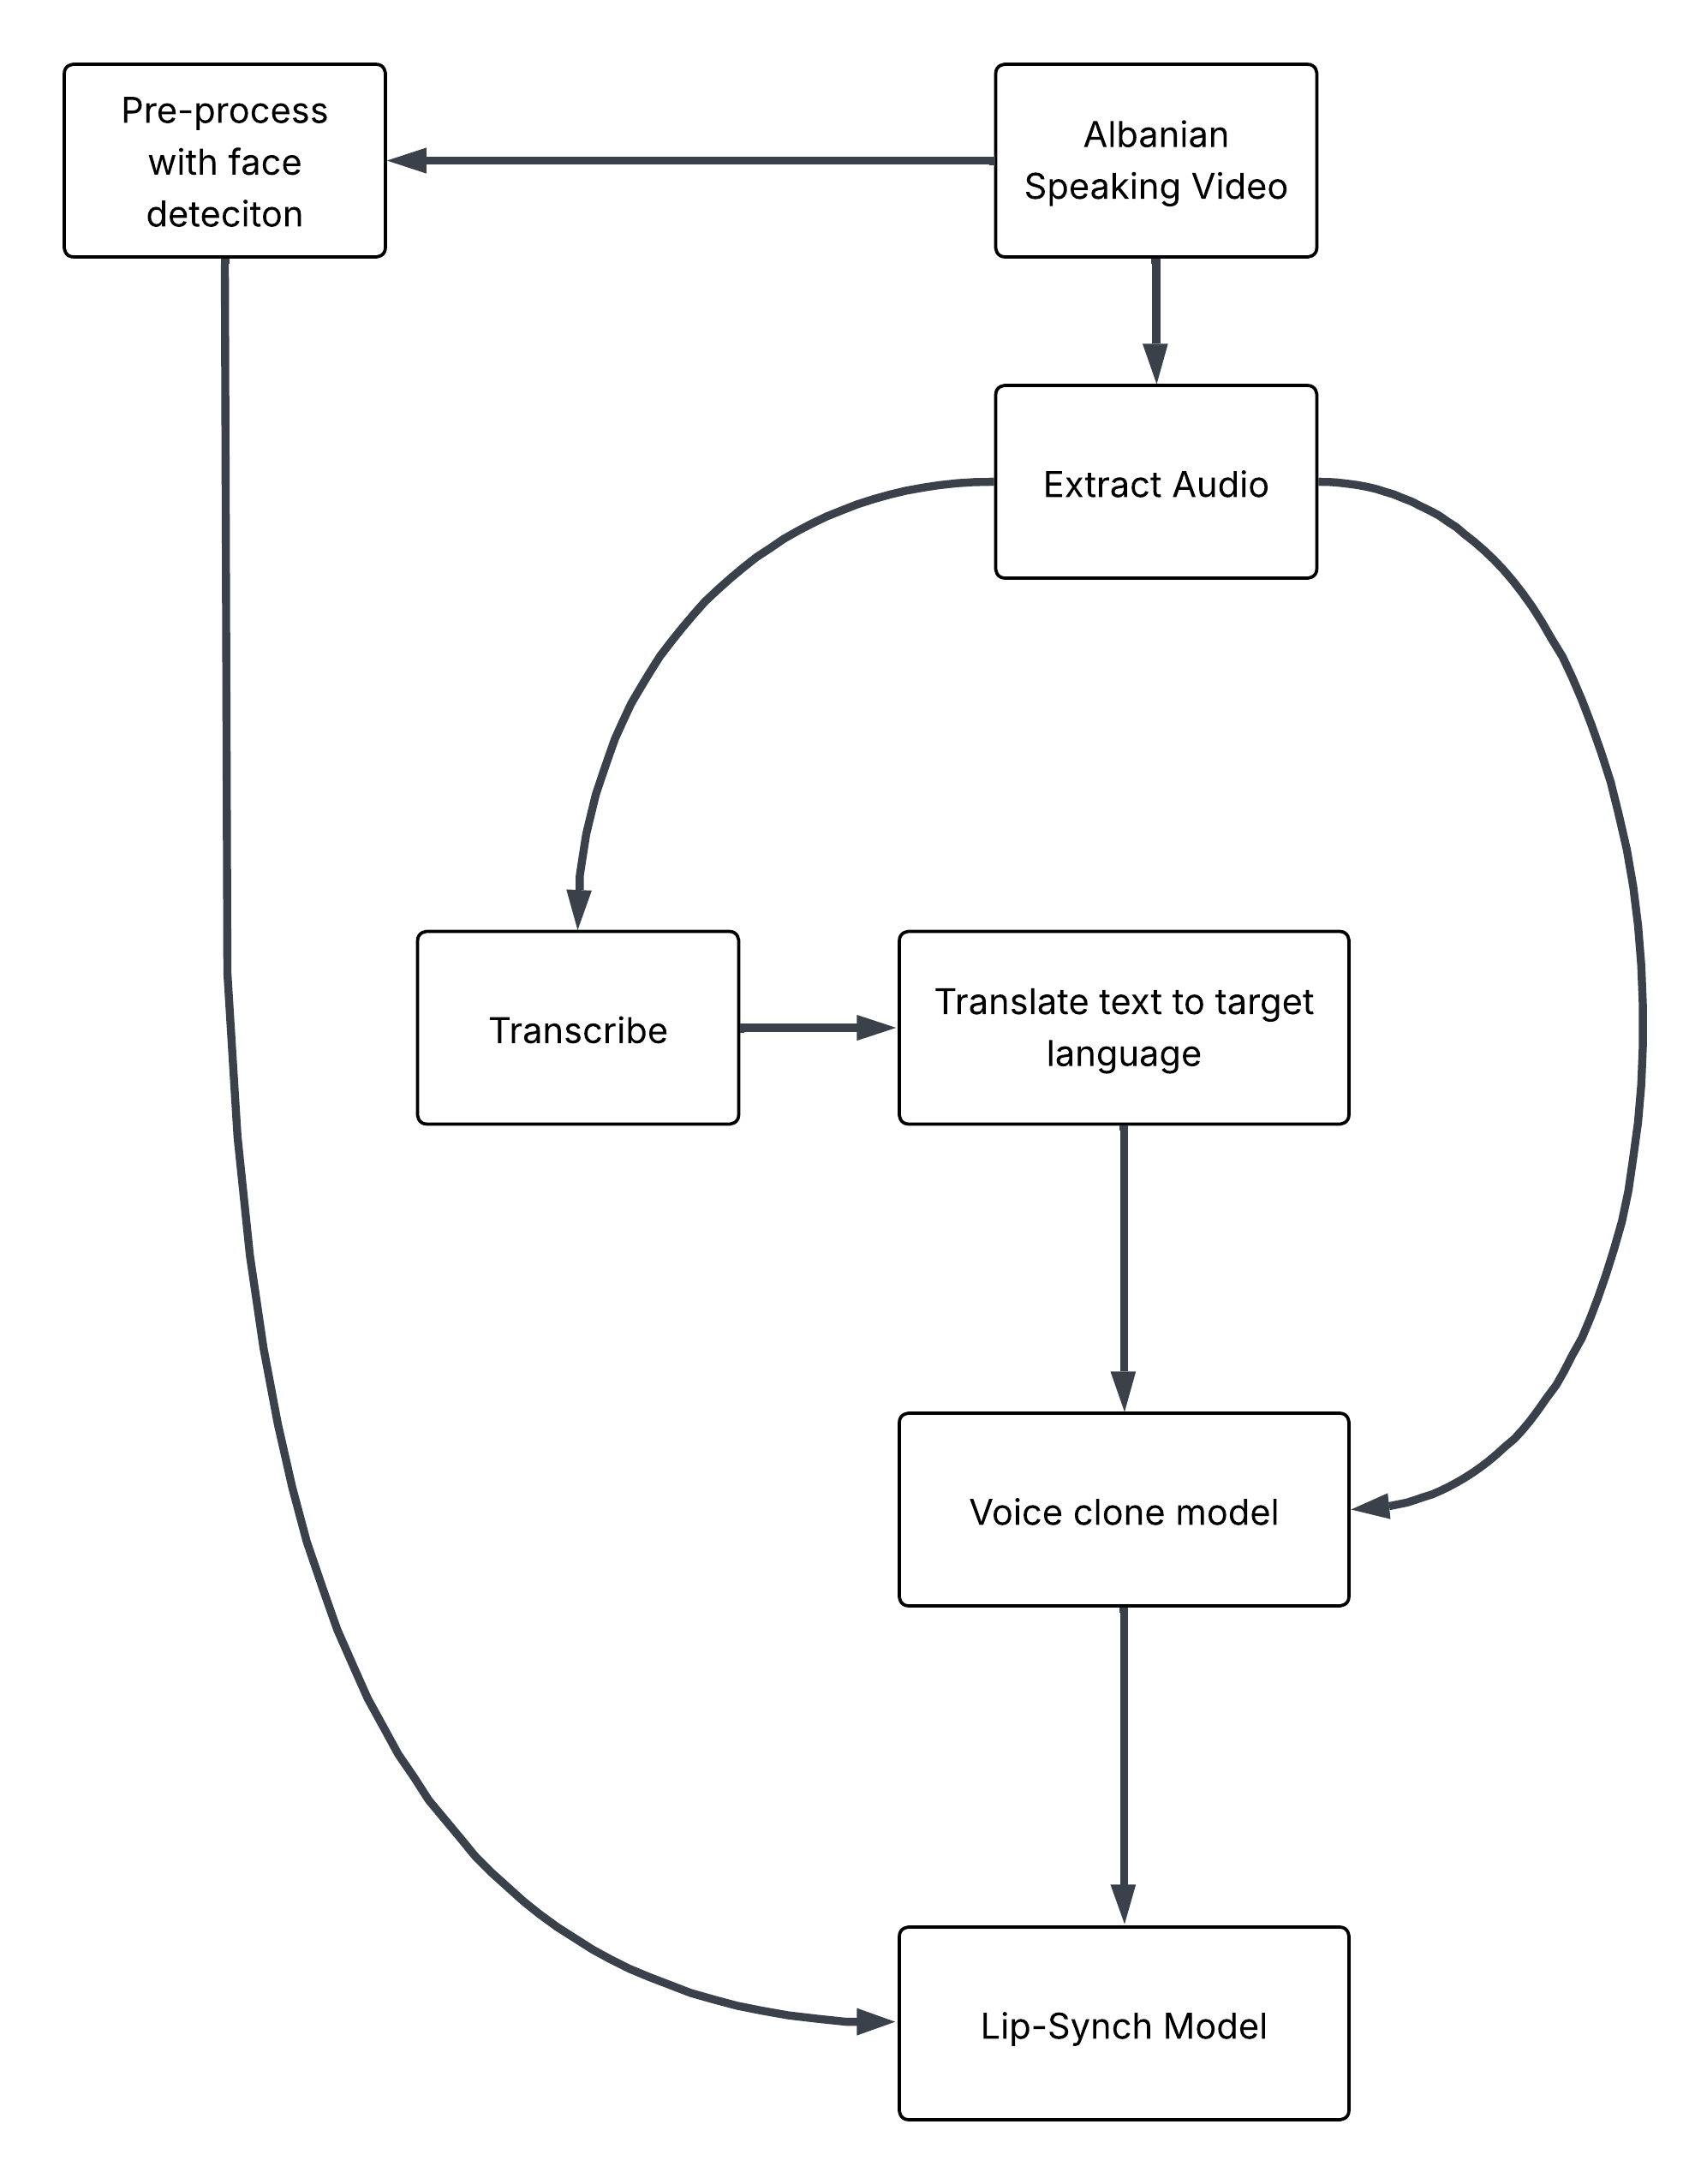
\includegraphics[width=0.5\textwidth]{images/work-flow.png}
    \caption{Work Flow}
    \label{fig:work-flow}
\end{figure}

Audio was then extracted from the videos using ffmpeg package, Pulse Code Modulation, Signed 16-bit, Little Endian (pcm\_s16le), a lossless, uncompressed audio codec format, 16000hz sample rate and monophonic, meaning single audio channel.  which will be used for transcription and for the base of the voice cloning tool before inputing it into the final lip synchronization model. For the audio extraction ffmpeg library was used, and audio was extracted in a lossless codec, 16000hz sample rate and signed 16-bit Pulse Code Modulation (PCM), per Google Speech-to-text API documentation \cite{google_api_docs}.\\
The audio gets sent through an Automatic Speech Recognition model, converting spoken language into written text. and gets saved in a text file, each line contains the name of the file transcripted and a colon separates it from the text. After several tests of three models, Google Speech to Text Chirp 2, Kushtrims and Neura, the latter one was selected as being the most accurate \cite{google_api_docs}\cite{kushtrim}\cite{neura}.\\
Transcripted text is translated to a target language that is supported by the voice cloning model. Using deep-translator python package and utilizing google translate as its core. Audio of the same file is used as reference to make a voice clone using OpenVoice, in the target language, a check is made if the cloned output is longer or shorter than the reference audio\cite{openvoice}. Another clone is made with the speed of the audio modified to be as close as possible to the original. OpenVoice offers emotion and accent cloning offering flexible voice control. The translated text will be used as the base of what the voice clone should output. OpenVoices Zero-shot cross-lingual voice cloning can generate speech that can be not present in the multi-lingual training dataset used by the model. There is "native" support and generalisation of voice clones. The native support is offered for languages like english, spanish, french, chinese, japanese and korean in the second version of OpenVoice.\\
The reference video is processed to be cropped in a 512x512, 25 frames per second format with the face centered, this was made using a face detection model which would detect faces in every frame of the video, from there we take the center and crop accordingly. Googles mediapipe framwork was used for the face detection task \cite{GoogleFaceDetector}. This format is a pre-requisite before inputting videos into the final lip-synching model.  Pre-emptive tests were done on the videos to see if the face detector worked as intended and could detect a face in every frame of the videos. 

After translating, the translated text and the original audio are used to make the voice clone. We need the original audio of the transcript because of emotions displayed in the audio can be used by the voice cloning tool.\\
Cloned voice and the original video from where the cloned voice was based on are then used to train the lip synchronization model. 

\textbf{One of the challanges of creating a lip synchronization in videos is the need for the lip movements to accurately align with a specified target speech segment, especially in multilingual and unconstrained environment. Visual data falling out of sunc with updated audio and inaccurate lip movements in target videos.}\\
CNN and Generative Adversial Networks (GANs) to create the lip movements that sync up, this combined with a Discriminator Network which would try and detect the GANs fake lip movements and real ones, pushing each other to get better.


\section{Audio transcription}
The first step of the project is extracting audio from the videos and this was done using the open-source ffmpeg package. Going by the suggestions for optimizing transcription quality through googles speech-to-text API documentation \cite{google_api_docs}, best practices, the audio was sampled at 16000 Hz, converted into a singned-integer bitrate, and in a lossless pcm\_s16le format. One group of audio files were made in a lossless format, signed 16bit PCM (linear16), 16000hz sampling rate. While the other folder, was made with the same codec but with 48000hz sampling rate.\\There is no open-source ASR model for Albanian language, and the amount of Albanian audio dataset is very low. Florijan (2023) managed to collect 40 hours of diverse accents, dialects and speech styles of Albanian audio, the purpose was to exceed an initial accuracy target of 45\% \cite{florijan-qosja}. This data was filtered out of 133 hours available, going through validation accuracy above 0.9 used for training. The base model used for this was Deep Speech 2 by Baidou \cite{deep-speech}, consisting of a combination of CNNs and RNNs. The model did managed to reach an accuracy of 46.3\%, passing the threshhold but the model is not suitable for real world application. To test if there was another better model suitable for the dataset used by Florijan we used the Whisper model by OpenAI \cite{openai_whisper}. At first we tested the biggest model out of the box to check its performance, There are seven distinct whisper models whos difference lies in the parameter size and support for english only. Whisper is trained on 680,000 hours of labeled audio data, 438,218 hours of English language only, 117,000 hours covering 96 languages, Albanian included, though it does not mention the amount of hours for each language. Audio was sampled at 16000hz in mono, similar to that of Googles documentation. Its English ASR performance was very close to that of a human. Models range from tiny (39 million parameters) to large-v3 (1550 million parameters) these models were tested, attempts to fine-tune the large-v3 model with the dataset from Florijan we fruitless as the training time for such large parameter model was over 177 hours on a RTX 3080Ti 12GB Nvidia graphics card and 32GB of RAM. All models were tested from ones with the biggest parameter to the smallest, the only model that we could feasibly train was the whisper-small with a little bit more than 8 hours. ASR systems are evaluated using a Word Error Rate (WER) score, measuring the number of errors (substitutions, insertions and deletions) needed to transform the output of the ASR system into the reference transcript or ground truth. A lower WER score indicates a better performance in \ref{eq:WER} we can see the formula used for the calculation. The fine-tuned whisper-small model achieved a 61.52\% WER, not usable in any application. Testing the accuracy of the whisper-large-v2 model as a baseline reference without any fine-tuning resultet in a 55.1\% Word Error Rate (WER) accuracy, the larger whisper-large-v3 model did not have much change and managed to score a 49.45\% WER, both of these not up to par. Facebooks Wav2Vec2 baseline model with 960 hours of training data was tested and managed to achieve a 97.74\% WER \cite{facebook-wav2vec}. 

\begin{equation}
\label{eq:WER}
WER = \frac{S + D + I}{N} = \frac{S + D + I}{S + D + C}
\end{equation}

Where:
\begin{itemize}
    \item S is the amount of substitutions,
    \item D is the amount of deletions,
    \item I is the amount of insertions,
    \item C is the amount of correct words,
    \item N is the amount of correct words.
\end{itemize}

From this point onward the search continued into closed systems, offered comercially. Googles Speech to Text API offered support for Albanian language and had free credits for first time user. Their system gives a confidence score for each transcription section and confidence score in individual words aswell. After transcription, a subtitle file format was also available to check the timings of when each word or sentence is spoken, this is an increadibly usefull feature as we could use it to cut the videos into smaller chunks as Pawar et al. (2024) experienced accelerated training process and improved performance when utilising a "vVISWA" dataset composed of isolated words \cite{PAWAR2024100084}. In the first test Googles Speech to Text API, using Chirp 2 as a model, managed to achieve a WER score of 10.7\%. Kushtrims model based on the whisper-large-v3-turbo and fine-tuned with 200 hours of curated Albanian audio with diverse dialect, hosted on the Hugginface Spaces, the model weights were not opensource, nor was the dataset used for the training \cite{kushtrim}. It did not offer a confidence score nor a SRT file with audio timings.The model could be accessed for inference using the API available from Gradio, which is how the transcriptions were processed, however the model was quite slow in times as more than one individual would try to transcribe audio at the same time, increasing the transcription time a lot, in some cases taking more than three hours for twelve seconds of audio. At a later point the model was updated with an additional 100 hours of Albanian audio. Both versions of the model were evaluated, in table \ref{tab:firs_test} we can see the scores for all models, and Kushtrims managed to get a 16.46\% WER. The other ASR model tested was Neuras \cite{neura}, a comercially available product, we were granted access and free credits. Their website advertises the model as having a 93\% accuracy, which a bit of an underestimation on their part as it scored a 3.09\% WER which is equivalent to 96.91\% accuracy. The first set of audio files contained casual speech and did not have language that would be deemed difficult to understand or hear, testing was done for ten files, comparing the ground truth to the hypothesis file.\\
WER as a metric has its limmitations, from the formula we can see that the substitutions, deletions and insertions have the same weight. A minor misspelling might have the same weight as a word that completly changes the meaning of the sentence. It also doesnt take in consideration a mistake in letters inside a word. For example, the word "duket" was incorrectly transcribed as "duhet", in this case the whole word is a mistake. All unneccessary elements are removed, punctuation, making numbers into 123. The core of the WER calculation is finding the minimum number of edits needed to transform the hypothesis (transcription) text into the reference (ground truth) text. This is typically done using a dynamic programming algorithm, specifically the Levenshtein distance algorithm, applied at the word level.
\begin{table}[h!]
\centering
\caption{Error Analysis for Challenging Albanian Scripts}
\label{tab:firs_test}
\begin{tabular}{lccc|ccc|ccc}
\toprule
\textbf{File ID} & \multicolumn{3}{c}{\textbf{Neura}} & \multicolumn{3}{c}{\textbf{Kushtrim}} & \multicolumn{3}{c}{\textbf{Google API}} \\
\cmidrule(lr){2-4} \cmidrule(lr){5-7} \cmidrule(lr){8-10}
 & \textbf{S} & \textbf{D} & \textbf{I} & \textbf{S} & \textbf{D} & \textbf{I} & \textbf{S} & \textbf{D} & \textbf{I} \\
\midrule
File 1 & 0 & 0 & 0 & 2 & 0 & 0 & 1 & 0 & 0 \\
File 2 & 0 & 0 & 0 & 8 & 0 & 0 & 7 & 0 & 0 \\
File 3 & 0 & 0 & 0 & 27 & 4 & 3 & 14 & 17 & 1 \\
File 4 & 27 & 7 & 4 & 53 & 15 & 24 & 25 & 7 & 3 \\
File 5 & 2 & 0 & 1 & 31 & 3 & 7 & 18 & 7 & 6 \\
File 6 & 0 & 0 & 0 & 6 & 0 & 0 & 2 & 0 & 0 \\
File 7 & 0 & 0 & 0 & 12 & 2 & 6 & 13 & 2 & 6 \\
File 8 & 0 & 0 & 0 & 6 & 0 & 1 & 4 & 0 & 0 \\
File 9 & 2 & 0 & 0 & 12 & 0 & 3 & 11 & 0 & 5 \\
File 10 & 2 & 0 & 0 & 10 & 3 & 2 & 5 & 2 & 0 \\
\midrule
\textbf{Total Errors} & \textbf{33} & \textbf{7} & \textbf{5} & \textbf{167} & \textbf{27} & \textbf{46} & \textbf{100} & \textbf{35} & \textbf{21} \\
\textbf{Overall WER} & \multicolumn{3}{c}{\textbf{3.09\%}} & \multicolumn{3}{c}{\textbf{16.46\%}} & \multicolumn{3}{c}{\textbf{10.70\%}} \\
\bottomrule
\end{tabular}
\end{table}

A second test was made reading along a script made with the purpose of being a difficult dialog. Five new videos were created, audio extracted and we tested Googles Chirp 2, Kushtrims and Neuras model as having the best results for a further analysis. Table \ref{tab:wer_hard} shows the results from the tested audio, very different results shown from the first test, Neuras accuracy dropped close to their advertised numbers, Kushtrims model was the one that moved less, although we have to keep in mind that this was the model with 300+ hours of training data, dispite this the models performance decreased. An anomaly was detected with Kushtrims model output because the number of Insertions is 52, in the transcription there were added words "Piii" after the end of the audio file which was not present in the other models. Removing these anomalies the models performance improves to 13.01\%, the number of insertions dropped from 52 to 30. Googles Chirp 2 had the best results, achieving a 5.17\% WER score, this could be the result of having a larger and more diverse dataset compared to Neuras model which might have more audio content with everyday speech rather than scienfic language.
\begin{table}[h!]
\centering
\caption{Second Analysis WER score}
\label{tab:wer_hard}
\begin{tabular}{lccc|ccc|ccc}
\toprule
\textbf{File ID} & \multicolumn{3}{c}{\textbf{Neura}} & \multicolumn{3}{c}{\textbf{Kushtrim}} & \multicolumn{3}{c}{\textbf{Google API}} \\
\cmidrule(lr){2-4} \cmidrule(lr){5-7} \cmidrule(lr){8-10}
 & \textbf{S} & \textbf{D} & \textbf{I} & \textbf{S} & \textbf{D} & \textbf{I} & \textbf{S} & \textbf{D} & \textbf{I} \\
\midrule
File 1 & 3 & 0 & 1 & 4 & 0 & 0 & 4 & 0 & 0 \\
File 2 & 8 & 0 & 1 & 4 & 0 & 0 & 4 & 0 & 0 \\
File 3 & 5 & 0 & 0 & 6 & 2 & 52 & 2 & 17 & 1 \\
File 4 & 5 & 1 & 1 & 4 & 1 & 1 & 5 & 1 & 1 \\
File 5 & 5 & 0 & 1 & 6 & 0 & 1 & 2 & 0 & 2 \\
\midrule
\textbf{Total Errors} & \textbf{26} & \textbf{1} & \textbf{4} & \textbf{24} & \textbf{3} & \textbf{54} & \textbf{21} & \textbf{1} & \textbf{3} \\
\textbf{Overall WER} & \multicolumn{3}{c}{\textbf{7.08\%}} & \multicolumn{3}{c}{\textbf{18.49\%}} & \multicolumn{3}{c}{\textbf{5.17\%}} \\
\bottomrule
\end{tabular}
\end{table}

Implementation of Googles API was the most challanging of the three models, as there were many different configurations, and the results varied when accessing it through the API. While Google's web UI offered more consistent transcriptions, the process required manual effort. Having the better accuracy of all tested models on the majority of the dataset and because of the nature of the audio content of the dataset being conversational language, Neura was chosen as the transcription model to go forward with the project. \textbf{Later tests on Kushtrim model show a lot of errors on the base 63 audio file, repetions of words. Not sure if it should be included.}

\section{Translation}
Python package deep-translator was used to translate the text from the ASR model to the target languages. Deep-translator is a library that offers multiple translation models such as Google Translate, DeepL, ChatGPT and Microsoft Translator. ChatGPT requires an API key to make use of the Large Language Model (LLM). For our usecase, Google Translate was used as it is free and offers a good accuracy.


\section{Voice Cloning}
Voice cloning is a subtask of speech synthesis, using deep learning to create speech imitating a specific voice. Prioritizing the preservation of the identity of the target speaker. Modern systems use a modular architecture to achieve realistic speech synthesis that replicates a target speaker's voice \cite{Real-time_voice_cloning_system}. Similar to lip-synch architectures, voice cloning also uses CNNs, GANs, Variatonal Autoencoders (VAEs), DIffusion Probabilistic models (DPM), RNNs and Transformer-based Models \cite{voice-cloning-survey}. We characterise voice cloning into several approaches, speaker adaption where we fine-tune a Text-to-Speech (TTS) model to replicate a specific user's voice using limited data \cite{voice-cloning-survey}. Few-Shot Voice Cloning (FS-TTS) follows the concept of the speaker adaption but specifies the amount of data required as it typically ranges from a few seconds to a maximum of five minutes. Zero-shot Voice Cloning (ZS-TTS) differs from the first two because it does not require fine-tuning for the TTS model. Instead it uses a speaker encoder which uses a short audio clip to generate speech with voice characteristics similar to the reference waveform \cite{voice-cloning-survey}. Multilingual Voice Cloning focuses on TTS systems that can support multiple lanuages while maintaining speaker's characteristics. Subdivisions of multilingual voice cloning are cross-lingual which allows the model to clone a reference voice and generate speech in a new language even if it was not largly present in the dataset. Intra-lingual are models with voice cloning within the same language. The NAUTILUS system from \cite{NAUTILUS} has the ability to clone untranscribed speech, using a small amount of untranscribed speech, cited as about five minutes. Experiments coparing performance with different amounts of adaptation data show that Mean Opinion Score (MOS) for naturalness and similarity can improve significantly from five seconds to 15 seconds of untranscribed audio, plateauing or showing only minor improvement beyond that (e.g. 30 or 60 seconds)\cite{Unified_system_for_Voice_Cloning_and_Voice_Conversion}. Noisy audio can negatively impact the quality of generated speech, a real-time voice cloning system notes that generated speech can have low intelligibility due to artifacts, such as murmurs, hums, or noisy audio \cite{Real-time_voice_cloning_system}. 
Because of different trainning and test datasets different reasearch focus on metrics such as speaker similarity, speech naturalness, intelligibility. or computational efficiency. Azizah (2024) used WER and Character Error Rate (CER) to measure the accuracy of models, using Whiper to generate text from the speech and comparing it with the reference text \cite{zero-shot-voice-cloning}. This method of evaluation is used by several other models to measure their intellegibility \cite{harminizaion-of-voice-cloning}\cite{chen2021v2cvisualvoicecloning}\cite{NAUTILUS}\cite{zero-shot-voice-cloning}. User opinions, surveys, interviews, social media analysis, AB preference test, Degradation Mean Opinion Score (DMOS), these are all subjective measures and used is several models evaluation, because in the end the voice is made for humans to hear. Yemin et al. (2025) which created a foundation model for real-time autonomous interaction and voice role-play \cite{viola-voice-role-play}. OpenVoice acknowledges the inherent difficulty in objective numerical comparisons across many different studies due to a huge variety of datasets, scales, and core functionalities. Using the translated text into the language of our choice we can then try and use a voice cloning model to make the voice dubbing. A lot of models were available for this task, Nari Labs released Dia \cite{Dia}, Chatterbox from ResembleAI \cite{chatterbox}, OpenVoice \cite{openvoice}, Viola \cite{viola-voice-role-play}. Some models offered more options about voice control, OpenVoice offers tone color and style from a reference speaker, emotion, accent, rhythm, pauses and intonation. Chatterbox offers different values of exaggeration, pace and temperature. Pacing or audio speed is very crucial in our project because of the differences in length of the reference audio and the output audio in the target language may be shorter or longer. Chatterbox is a new Voice Cloning model, its main support is for English language and it is quite limited in duration as it cannot do more than 35-40 seconds before starting to lose quality. It offers options to control the voice cloning with CFG/Pace, random seed nad temperature, on the Huggingface Space it only allows for 300 characters maximum input which limits our abilities quite a lot. Trying different values for the pace does very little to the change of audio length as it mostly changes to although it is more natural than others, it still has issues as if the values of the pace change too much or the exaggeration value changes too much it can create artifacts, moments of silence of up to 4 seconds that did not exist in the reference audio. Chatterbox includes a built-in PerTh Watermarking for responsible AI usage.  


Voice cloning can be of help to those with speech disability, as most of the models are trained on normal human voices. Azizah (2024) presented zero-shot voice cloning Tacotron-2 based TTS for people with dysphonia, the choice for zero-shot was because of the impossibility of training a TTS model using data from people who suffer from dysphonia \cite{zero-shot-voice-cloning}.\\
Ethical questions regarding Voice Cloning are paramount, primarily surrounding individual rights, potential for misuse and societal impact. In a hugly digitalised world where people share a lot of video content online they might not know that their voice can be collected and used for trainning, raising questions about privacy infringement and data protection \cite{harminizaion-of-voice-cloning}. Issues with identity and authenticity will rise as synthetic voices become increasingly natual sounding. Potential for misuse and harm, malicious exploitation of voice cloning for deception, fraud, manipulation and financial scams \cite{threats-of-voice-cloning}. 


\section{Lip synch model}
Before deep learning lip-sync was achieved using viseme-based and rule-based system, mapping phonemes to corresponding visual mouth shapes. These methods were more commonly used in cartoons as they lacked the realism and fluidity of natural speech \cite{automatic-lip-synch-methods-in-games}\cite{https://doi.org/10.1002/vis.4340020404}\cite{computers14010007}. Figure \ref{img:viseme} shows the visemes for letters a, b, c, d, e, ë, f, g, j in the Albanian alphabet. Since every letter has a uniques sound in the Albanian language. 
\begin{figure}[h!]
    \centering
    \includegraphics[width=0.5\textwidth]{images/visemes.png}
    \caption{Visemes}
    \label{img:viseme}
\end{figure}
Movement of the lips depend on the emotions of the speaker, researchers noticed that lip-syncing and broader facial animation are not the same across different emotional states like anger, sadness, happiness, surprise, fear etc. \cite{audio-driven-facial-animation}. These emotional nuances can indeed be learned and trained by advanced models to be cloned or mimiced in generated outputs \cite{multilingual-lip-sync} \cite{mimitalk}. Human evaluators consistentyl assess wether the generated output matches the emotional tone implied by the audio and they look for smooth transitions between emotinal expressions. Models like EmoTalk and EMOTE explicitly work to extract the emotions from the audio and integrate the effects of both emotion and speech to produce more nuanced emotional representations in 3D animations \cite{audio-driven-facial-animation}. 

GeneFace++ is an improved version from GeneFace \cite{geneface} \cite{ye2023geneface++}, it progressed on three key areas, Audio-to-Motion Module, enhanced robustness (Landmark locally linear embedding), and improved efficiency (Instant Motion-to-Video Module). In Figure \ref{geneface} we can see the structure of the model, section (a) shows the full structure of the pipeline, from the inputed audio, training the Pitch-Aware Audio2Motion, Landmark LLe projection and the instant Motion2Video at the end \cite{ye2023geneface++}. These additions aim to address the limitations of generalizability, video quality and system efficiency observed in the original GeneFace model. The nature of the architecture of the model, having a 3D model of the face can help with issues of Preparing the dataset before training was needed, the videos needed to be scaled into 512x512, mediapipe \cite{GoogleFaceDetector} was used as a facedetector.

\begin{figure}[h!]
    \centering
    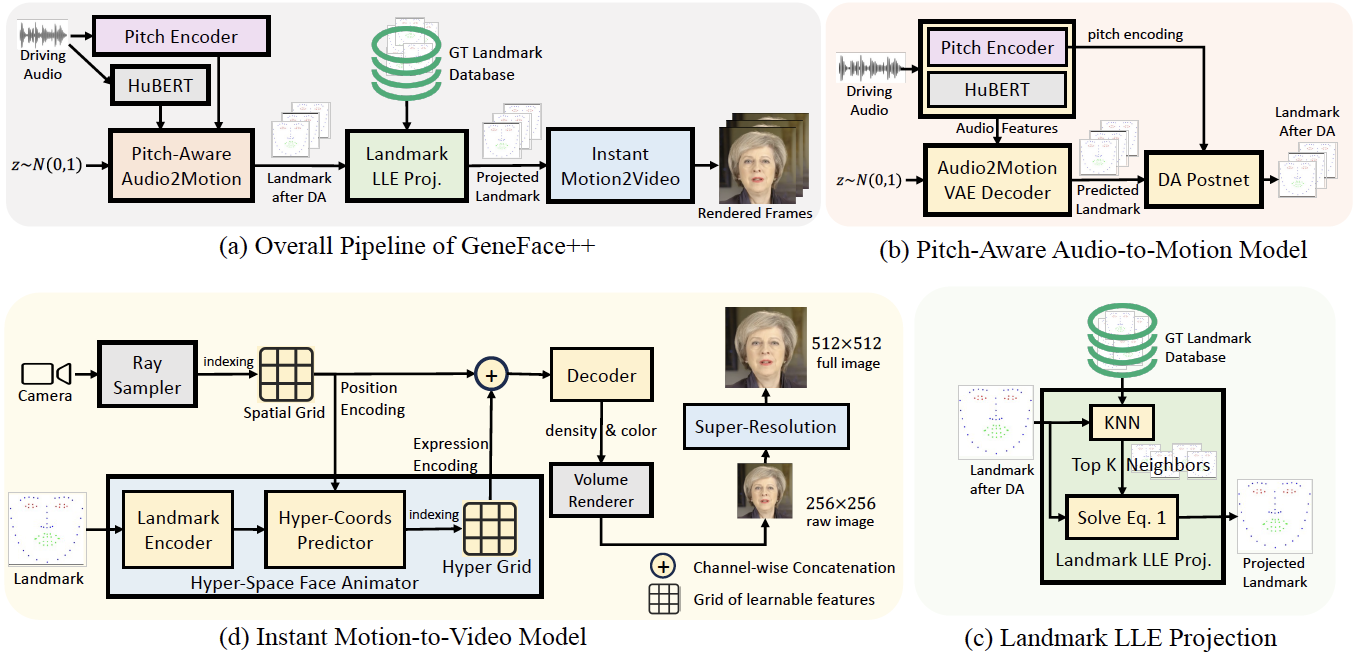
\includegraphics[width=0.5\textwidth]{images/geneface++.png}
    \caption{GeneFace++}
    \label{img:geneface}
\end{figure}

An early issue came up as the face detector could not detect any face in all frames of the video, this was the same for all the videos in the dataset. Getting the metadata information out, we observed that videos had a rotation of \-90 degrees. Mediaplayer applications would see this flag and add a 90 degree clockwise rotation to show the video correctly, but the face detection software would go through raw pixel data thus ignoring the flag and getting a sideways face. Most face detection models train on upright faces making them fail when faced with faces sideways or face-down. When applying a clockwise 90 degree rotation on the raw pixels of the video and changing the rotate flag to 0, the videos would come out as sideways, this might be beacuse ffmpeg might apply a correction rotation before the rotate command, thus we needed to apply two ffmpeg commands, one to rotate +90 degrees clockwise and set the rotate flag to 0, and the next command to rotate the video again with a -90 degrees counter-clockwise.
The "min\_detection\_confidence" variable was also lowered from 0.7 as a default option to 0.6, with the new value the model was able to detect faces. Next step for processing data was audio feature extraction, using mel, f0, hubuert or esperanto. We extract individual image frames from the processed video, using lm2d\_mediapipe we extract 2D facial landmarks from the video frames. These 2D landmarks are crucial for fitting a 3D Morphable Model (3DMM) in the next step. Fitting 3DMM, we take 2D facial landmarks and "fit" them in a 3D Morphable Model to the person's face in each video frame. This makes the model more suitable for usage on a specific person as we are training the NeRF model for the head and torso. This fits our dataset more as the videos are of a single person. The last step is about packaging and organizing the generated data into a binary format that is optimised for efficient loading and training of the subsequent neural network model. Handling of different audio and video lengths, although not specifically mentioned in the research we can infer based on the architecture, the model would likely continue to generate facial motion based on the remaining audio. We can test to see how the model performs with a different head and torso NeRF model using the one pre-trained by GeneFace++ or train them ourselves before inferencing. GeneFace++ is a model that works by training the Audio2Motion model which comes pre-trained in this case. We need to train Motion2Video renderer ourselves after the data has been prepared. Training is done for the head model and the torso model separatly. Finalizing all of these we can go to inference, we used the longest video in the dataset (five minutes) to train the head and torso model. The model for the head was stopped after one hour and 30 minutes after observing the lack of change in the total loss value. From Figure \ref{img:head_model_training} we can see on graph Total Loss over Steps that the minimum value it reached (1.12 total loss) was at 15,000 and 20,000 steps. After it continued to fluctuate with a maximum of 20 and an average of 15.48. Mean Square Error Loss (MSE) and Super-Resolution Mean Squared Error Loss (SR MSE) go down at the begining of the steps and stay constant, while the Lambda Ambient has identical values to that of the total loss, this makes it the main factor contributing to the total loss value. 

\begin{figure}
    \centering
    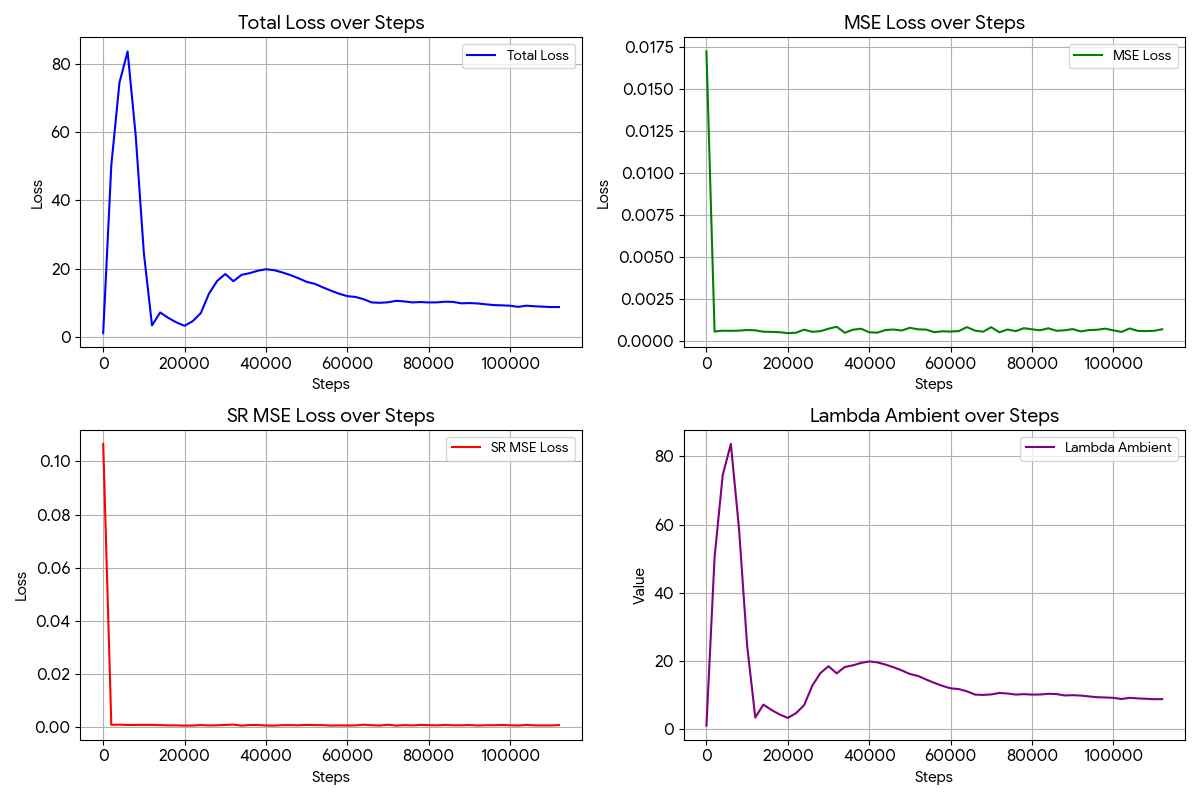
\includegraphics[width=0.5\textwidth]{images/head_training_loss.png}
    \caption{Head model training}
    \label{img:head_model_training}
\end{figure}

The models configuration was training for 250,000 steps. After 1 hour and 30 minutes of training the results were as shown in Figure \ref{img:training_loss}. The total loss drops to the lowest value of 8.6979, after 20,000 epochs and continues rising till 384 in step 90,000. In Figure \ref{img:mse_sr_mse_loss} we can see that MSE and SR-MSE keep going down consistently till step 30,000 where we can see fluctuations. The culprit of the high loss in our case is the lambda ambient loss, which we can see in Figure \ref{img:lambda_ambient_loss}, as the line for the lambda ambient loss fits perfectly with the line of our total loss. This value measures how well the model is handling the ambient (non-facial, background, or global lighting) aspects of the scene. Target ambient loss in the configuration files was changed from 1.0e-8 to 1.0e-6 which the authors say might be more suitable for men. 

\begin{figure}[h!]
    \centering
    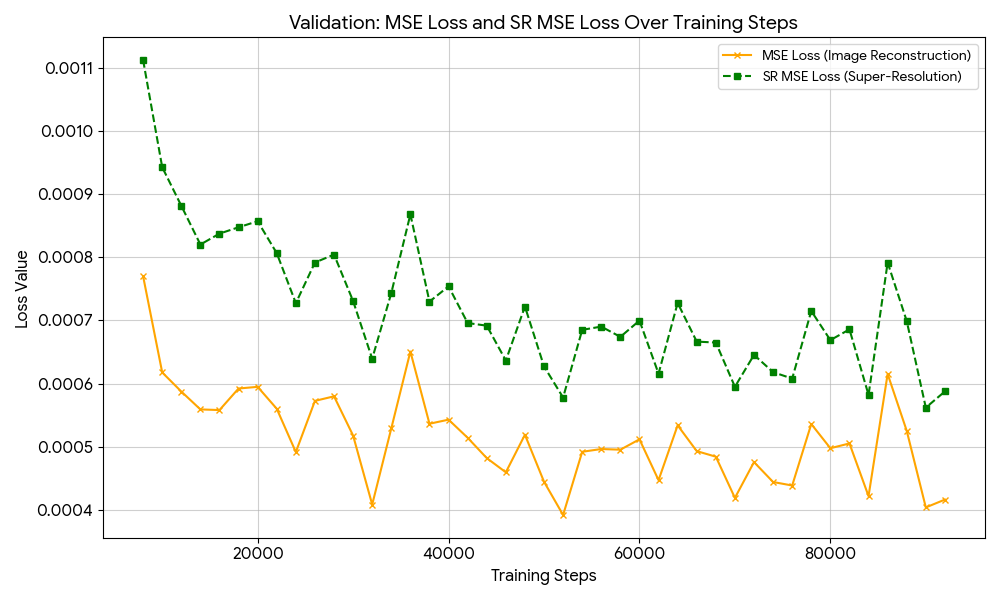
\includegraphics[width=0.5\textwidth]{images/mse_sr_mse_loss.png}
    \caption{MSE, SR MSE loss}
    \label{img:mse_sr_mse_loss}
\end{figure}

\begin{figure}[h!]
    \centering
    \begin{minipage}{0.45\textwidth}
        \centering
        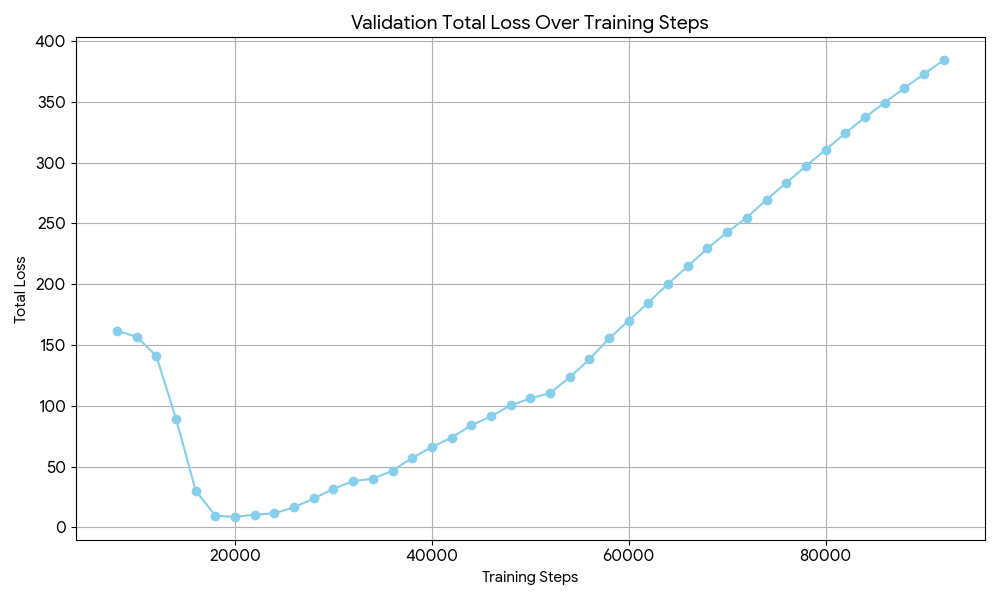
\includegraphics[width=0.8\linewidth]{images/training_loss.png}
        \caption{Total Loss}
        \label{fig:training_loss}
    \end{minipage}\hfill
    \begin{minipage}{0.45\textwidth}
        \centering
        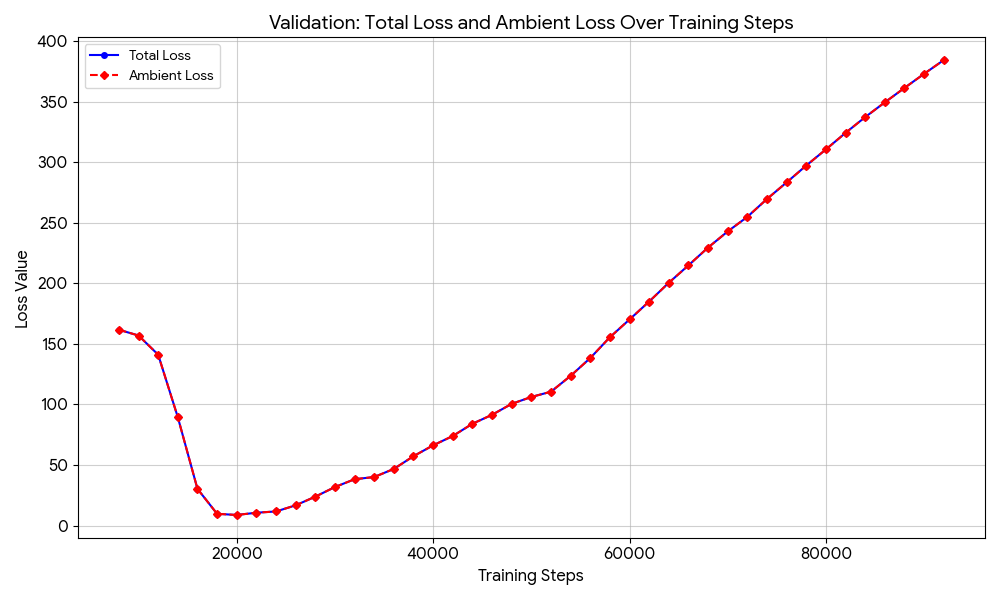
\includegraphics[width=0.8\linewidth]{images/lambda_ambient_loss.png}
        \caption{Lambda ambient Loss}
        \label{fig:lambda_ambient_loss}
    \end{minipage}
    \caption{Results from head model training}
    \label{fig:first-head-training}
\end{figure}

After the changes the ambientloss values were as shown in Figure \ref{img:ambient_loss_v2}. MSE and SR-MSE loss values were as shown in Figure \ref{img:MSE_v2}. The model was trained for 198,000 steps before stopping as the loss values got below 0.001 as shown in Figure \ref{img:total_loss_v2}.

\begin{figure}[h!]
    \centering
    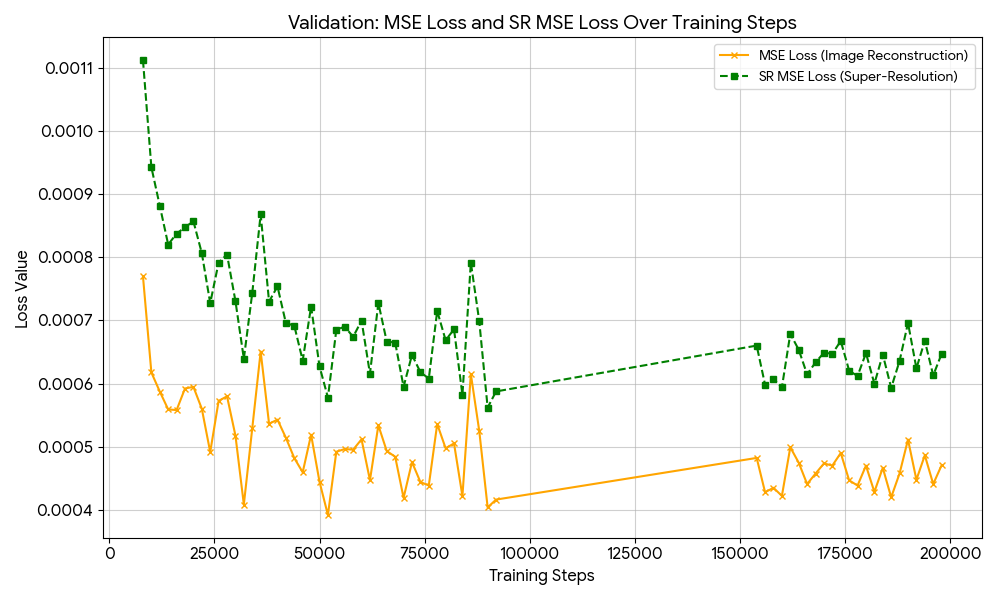
\includegraphics[width=0.5\textwidth]{images/MSE_v2.png}
    \caption{MSE second iteration}
    \label{img:MSE_v2}
\end{figure}

\begin{figure}[h!]
    \centering
    \begin{minipage}{0.45\textwidth}
        \centering
        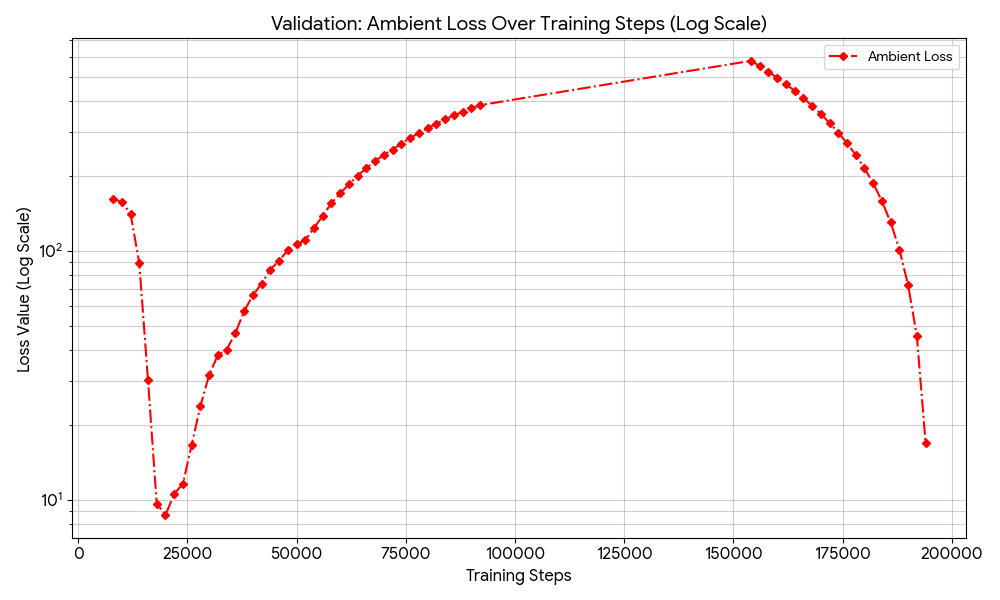
\includegraphics[width=0.8\linewidth]{images/ambient_loss_v2.png}
        \caption{Ambient loss second run}
        \label{fig:ambient_loss_v2}
    \end{minipage}\hfill
    \begin{minipage}{0.45\textwidth}
        \centering
        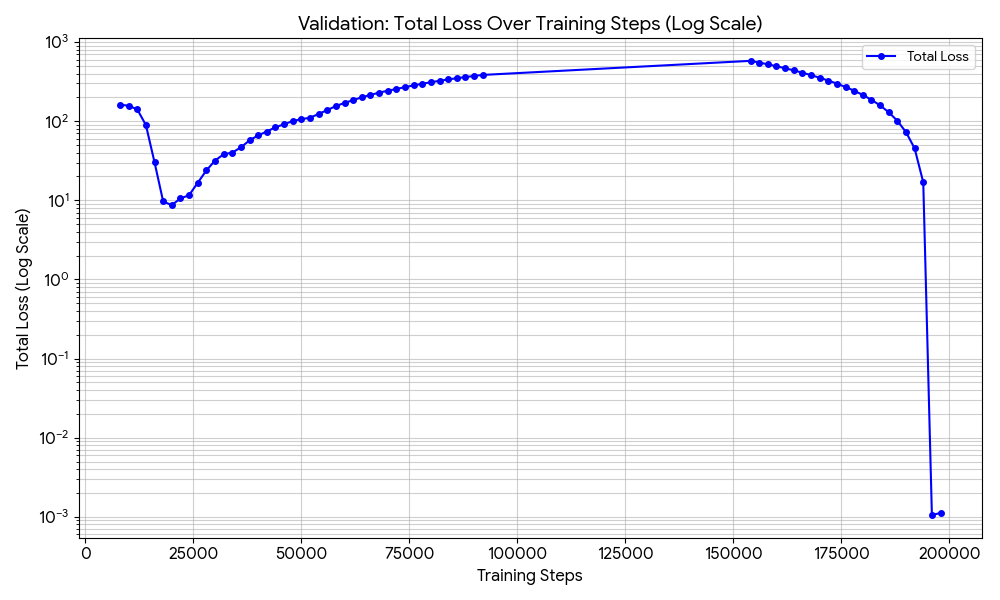
\includegraphics[width=0.8\linewidth]{images/total_loss_v2.png}
        \caption{Lambda ambient Loss}
        \label{fig:total_loss_v2}
    \end{minipage}
    \caption{Results from second training}
    \label{fig:second-training}
\end{figure}

The training of the Torso NeRF model is dependent on the performance of the pre-trained Head NeRF model. During the initial training of the Head NeRF model, suboptimal convergence behaviour rendered the resulting Head model unsuitable. Consequently, any Torso NeRF model trained using the badly optimised Head model is unreliable for the final generation pipeline.\\
A third training was done to the torso model after changes to the configuration files, lambda ambient value and eye blink dim changes from four to two. In Figure \ref{fig:validation_torso_total_loss} we can total loss per training steps, the lowest total loss value occured at step 34,000. The training was stopped at 46,000 steps as the total loss was not decreasing more. At 8000 steps the models total loss is 0.104, showing a slight decrease to a minimum of 0.0768 at 38,000, before rising slightly again. It is largly plateauing within the range of approximately 0.076 to 0.112. This means the models overall performance on the validation set is no longer significantly improving. 
\begin{figure}[h!]
    \centering
    \begin{minipage}{0.45\textwidth}
        \centering
        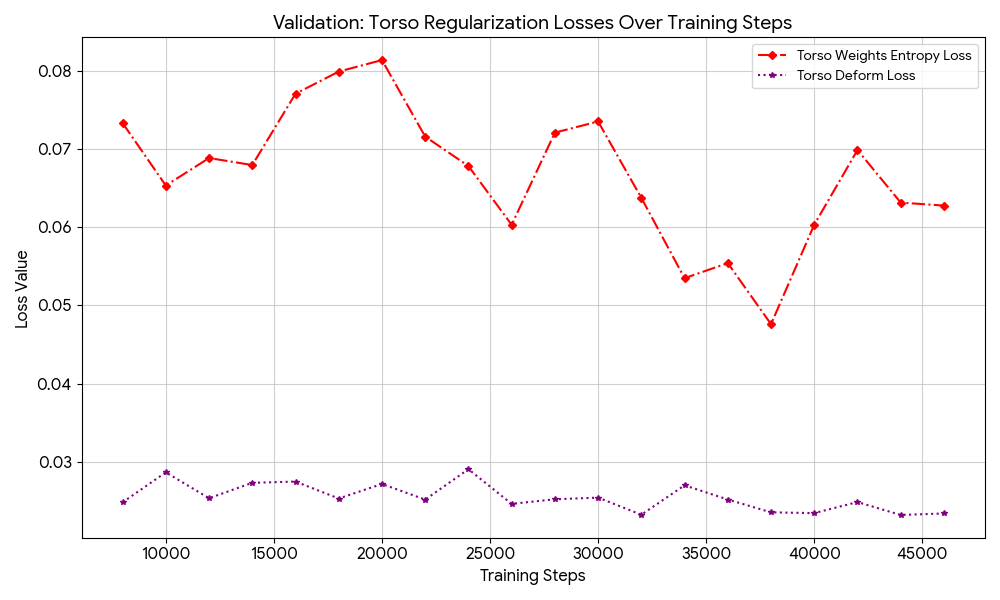
\includegraphics[width=0.8\linewidth]{images/torso_weight_entropy_loss.png}
        \caption{Weight Entropy loss}
        \label{fig:torso_weight_entropy_loss}
    \end{minipage}\hfill
    \begin{minipage}{0.45\textwidth}
        \centering
        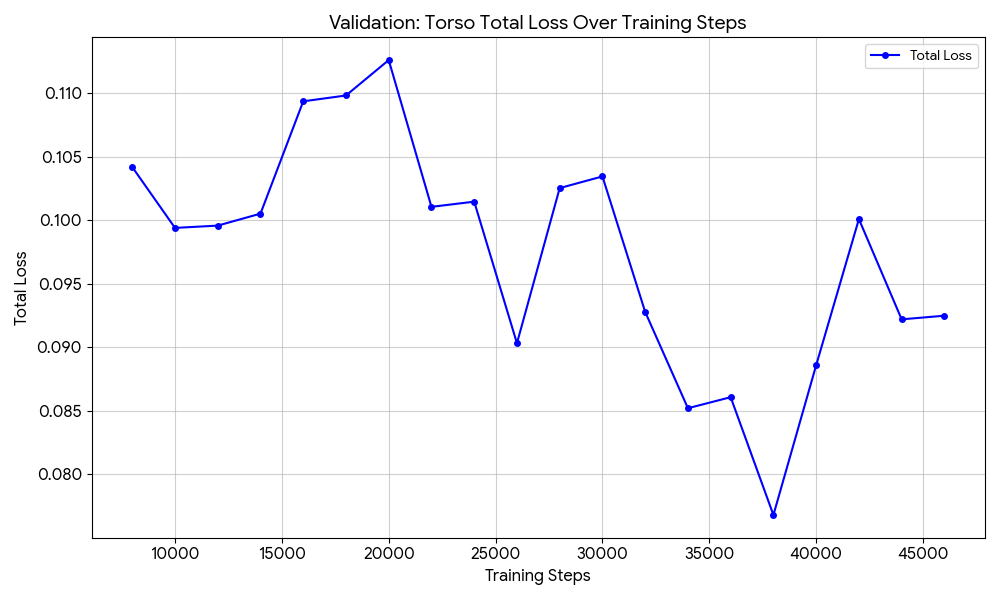
\includegraphics[width=0.8\linewidth]{images/validation_torso_total_loss.png}
        \caption{Validation Torso Total loss}
        \label{fig:validation_torso_total_loss}
    \end{minipage}
    \caption{Results from third torso model training}
    \label{fig:third-training}
\end{figure}

The first inference was run with the debug flag to check for any errors during the process, and Image \ref{img:first_inference} we can see the three parts, on the left we have the produced video, in the middle we have the landmarks for the face and lips, and on the right is the mask for the whole face. From the outputed video, we can observe the decrease in image quality, the face features were not very visible and the mouth was not moving as well copared to the landmarks and the mask, the last two were in sync with the audio provided for inference. The video lasted as long as the audio did, so we can conclude that GeneFace++ does shorten the video according to the audio length because of its architecture with the 3D model. This also means we can produce content with audio that is longer than the original video reference. Despite multiple tests we were not able to make the trained model on our dataset work as intended to create a clear lip-sync, the landmarks as shown in the debug faze, are synched but the overlapping face on the speaker was not able to replicate those. 

\begin{figure}[h!]
    \centering
    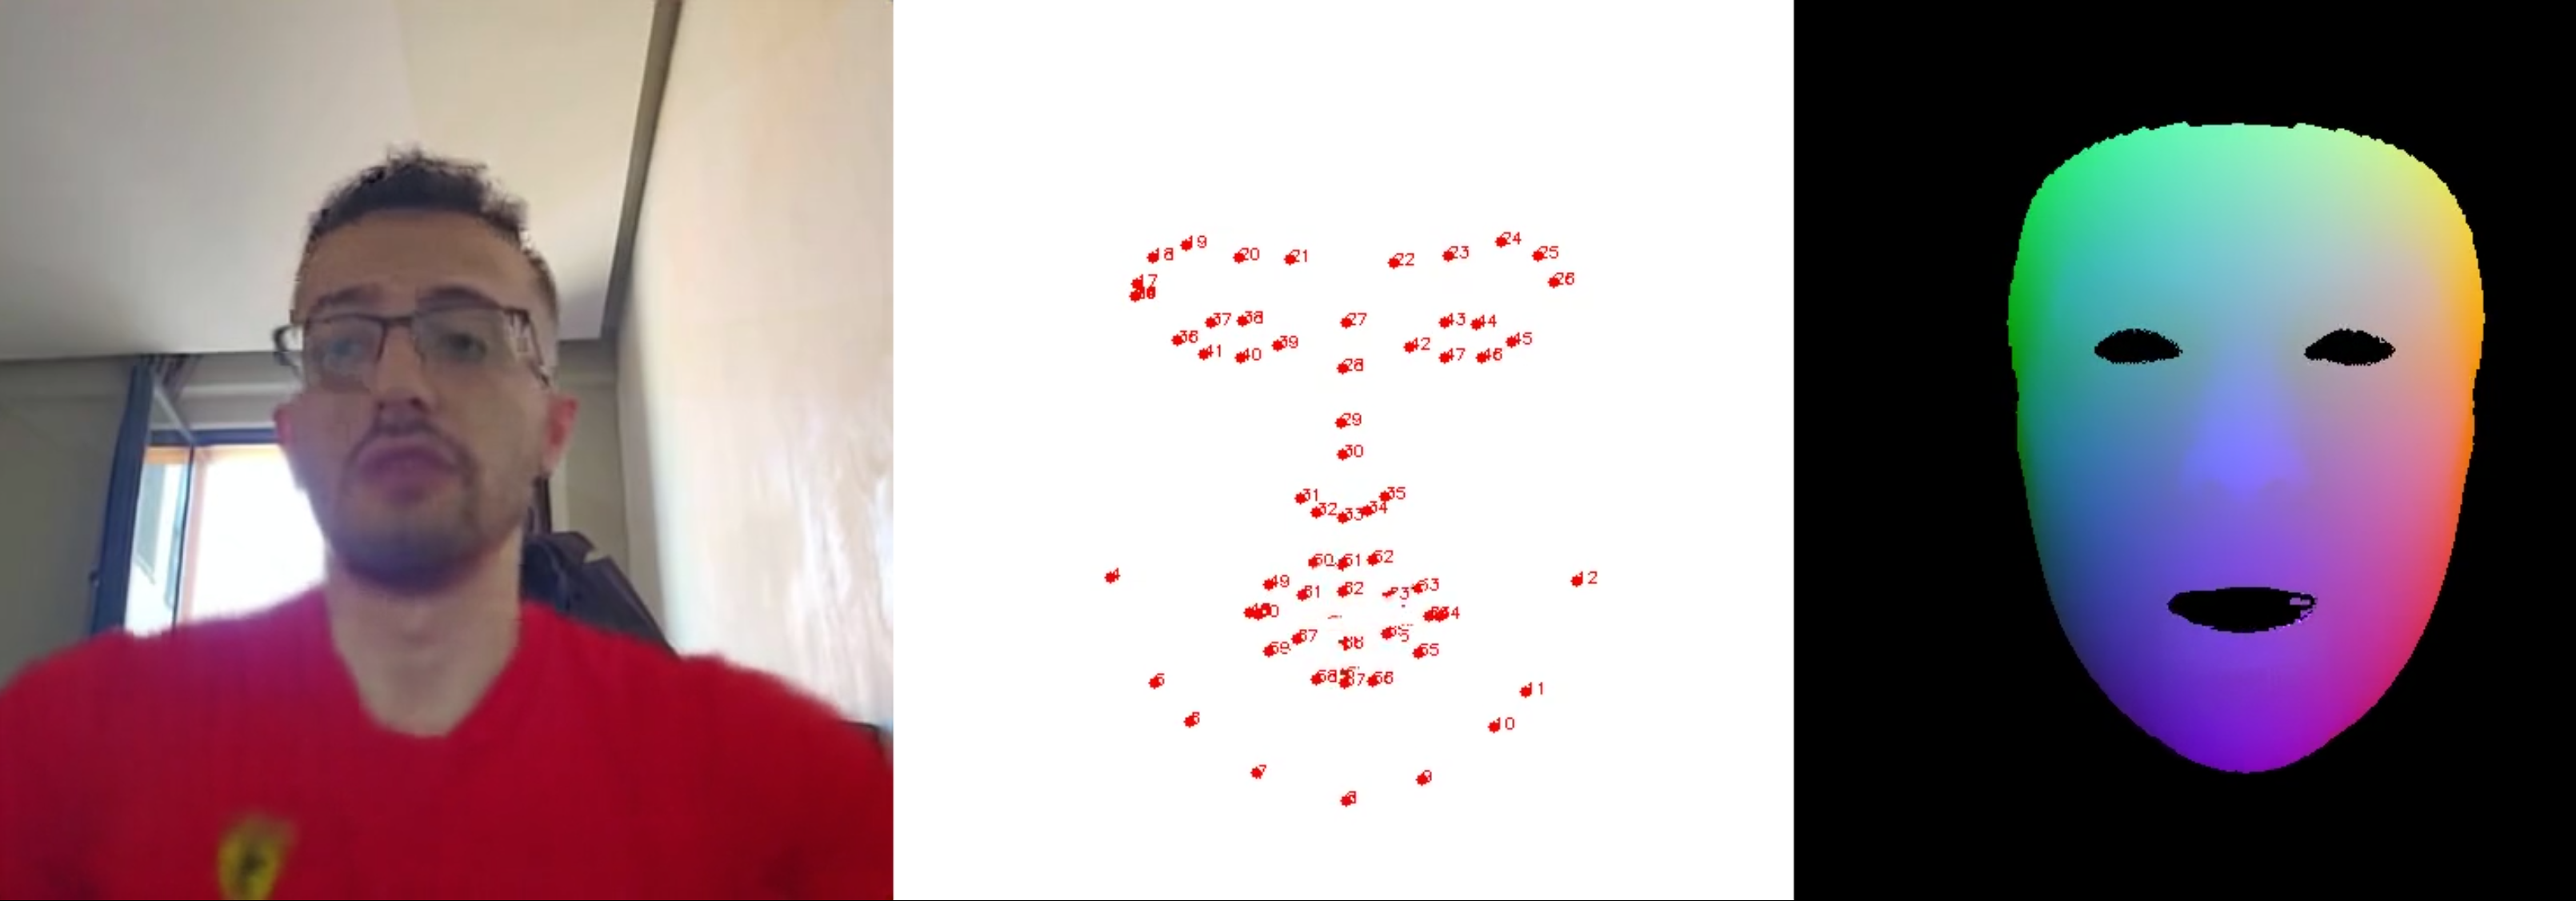
\includegraphics[width=0.5\textwidth]{images/first_inference.png}
    \caption{First inference}
    \label{img:first_inference}
\end{figure}



\section{Future improvements}
Creating an open-source albanian ASR model, using models like Kushtrims and utilizing the free credits from Google Speech-to-Text API, making use of the confidence score to save only audio that is above a certain threshold, to create a dataset that is more accurate and reliable.\\
An ASR model of the target languagecan be used to verify the accuracy of the voice cloning model, by comparing the transcribed text with the translated text, for this we would need the target language ASR model to be very accurate.\\
LLMs can be used to translate the text, and could be of help when faced with discrepancy in audio timing of the reference audio and the cloned audio. Making the text shorter while keeping the meaning of the text the same. Changing the text to be more suitable for the voice cloning model. When faced with text that is of Albanian dialect, LLM could be used to transform the text to be more suitable for the voice cloning model.\\


\section{Limitations}
The project is limited to only the Albanian language as such the dataset is comprised of only Albanian speaking videos. Lack of open-source ASR models, and freely available datasets that fit into our requirements of having the person speak Albanian clearly, and facing the camera. Human evaluation bias in voice cloning, which is subjective and can be faulty or biased. Storage and computational power requirements, both local storage and cloud storage. Using Huggingface Spaces was problematic because the speed of audio transcription changes based on the availability of resources as everyone can use it, similar situation for the voice cloning models tried.\\
While Kushtrims model does say it is trained on Albanian audio with dialects, traditional translation models are not able to handle dialects, thus leading to a bottleneck in the project.\\
Voice cloning models that could not produce audio more than 30 seconds created an issue in cases where the videos were longer than 30 seconds.\\
Different models had different ways to prepare the data for training, some models required the data to be in a specific format, creating a need to save the original data without changes then applying the format to create new data, increasing the amount of data stored. These differences create the need to make scripts to process the videos according to the format, and issues such as out metadata rotate flag might come up and need special solutions. Some models were limited on image quality or image size, Wav2Lip requiring downgrading to 720p video quality in cases where the computing power is not enough.\\
In unknown languages it would be hard to detect anomalies in voice cloned speech, sounding words longer than it should, cutting words in half, or making the words shorter than they should are issues that are hard to detect if you are not a native speaker. 

\subsection{Questions raised}
List of questions:
\begin{itemize}
    \item Do out lips move the same despite different emotions?
    \item Can we lip synch the same video with different emotions? Or just clone the video with the emotion expressed?
    \item How do we know if the transcription is correct programatically?
    \item How should the data be prepared for the lip-synchronization model?
    \item Video format, 30 frames per second or 25, quality of the video, resolution, etc.
    \item Audio format, mp3, lossless, bitrate, etc.
    \item How does the duration of video chunks used during preprocessing impact the performance of the final machine learning model, and what chunk length yields the best trade-off between information retention and computational efficiency?
    \item How are voice cloning models evaluated, as it feels like it should be done with a human evaluation and that is faulty most of the time?
    \item Which would be the best model for the lip-synchronization task based on the data we have?
    \item Best way to handle differences between original audio timing and the voice cloned sample timing. (slow down the voice? speedup)
    \item Is an LLM better than a traditional tool for translating? Neural Machine Translation (NMT) vs Large Language Models.
\end{itemize}
As for the optimal length of the video chunks, the study done by \cite{PAWAR2024100084} faced challanges with lengthy continuous speech, inlcuding time-consuming merging issues and potential overfitting. This was addressed by using the "vVISWa" dataset which contains isolated words or indepentent speech. This improved the performance of the model a lot and reduced overfitting. However Goncalves et al. (2024) using the LRS3 dataset containing short sentences averaging 3.42 seconds, found that using such short sentences could lead to a drop in translation quality \cite{lipsynchronydirectaudiovisual}.


List of challanges:
\begin{itemize}
    \item Low resources for the datasets in albanian, in video and audio.
    \item No open source models for the transcription of the audio from albanian.
    \item Voice cloning models being evaluated using a human evaluation and that is biased.
    \item Storage of data, both in the cloud and locally.
    \item Computing power, GPU, TPU, etc.
    \item Training time.
    \item If the spoken albanian is with a heavy dialect, an Albanian ASR trained with large number dialects is needed
    \item If the cutting of videos is not done correctly, it is possible to cut a word in half
    \item Translating the transcribed albanian dialect. How possible it is? NLP script transformation + translate*
    \item Voice cloning emotions.
    \item Video chunking first then transcription, or transcription (have to keep timings) then chunking - might be more possible and more cost effective than the NLP to find the problems in the language/chunked words but not for dialects.
    \item Could probably use the timings from google speech-to-text api (or any timings) to make the cuts since it offers that. Making the better option to be transcript first then cut/chunk second.  
    \item Multiple Ethical challanges
    \item NLP + basic quantized LLM for better albanian understanding and translation?
    \item 
\end{itemize}

List of improvements:
\begin{itemize}
    \item Better dataset, quantity and quality, diversity (age, gender, moustache, skin color, lip color- lipstick, ethnicity, also in this case, dialect)
    \item Separation of dataset into single word video for better model performance.
    \item Albanian ASR open-source model, google speech-to-text API is paid service, and Kushtrims uses huggingface spaces which is slow
    \item Comparison between Google Speech-to-text API and Kushtrim ASR
    \item Addition on an NLP to handle transcription errors
    \item NLP for dialect speech, to transform it into something that can be translated, maybe LLM is better in this case.
    \item Better voice cloning. More emotional expression
    \item Better face reproduction from the emotions of the voice clone.
    \item Real time lip-synch dubbing
    \item Separating the dataset into two groups the new dataset with videos close to one word per video and see the results of that and the original dataset with longer videos. 
    \item NLP can also be utilized in the audio length check, if we have too much of a difference in audio length, we could apply NLP-s to change the sentence into something shorter or longer but keeping the sentence about the same.
\end{itemize}

List of things to not forget to add:
\begin{itemize}
    \item Mention confidence score in google api, it also offered timings like SRT file
    \item Kushtrim first 63 videos were on 200 hours of dataset, and the next 5 "hard" videos were on 300 hours. There can be a slight comparison on the accuracy. Should retest it.
    \item Write about the changes in translation from NTL to LLM being better, keeping context etc.
    \item Mention the fact that there is no open-source Albanian ASR model, no large open-source free-use dataset either. 
    \item Lowering the confidence coeficient in the face detector as it was from 0.7 where it could not detect a face. no matter the image rotation and the issue with the -90 degrees in metadata. 
    \item Also playing with the close face or far face, 0 or 1 values.
    \item In our case with GeneFace++, we are scaling the video in a 512x512 with the face being the center, this make the video much smaller, if we wanted a larger video, we would need to save both frames, scaled with GeneFace++ applied and the uncropped and paste the applied frame into the bigger frame.
\end{itemize}

\bibliography{references}
\bibliographystyle{plain}

\end{document}